El framework elegido para implementar el servidor ha sido Flask~\cite{Flask}. Por este motivo, debido a su gran compenetración, se ha dedicido utilizar la herramienta para gestión de base de datos SQLAlchemy.
\subsection{Persistencia con SLQAlchemy}
SQLAlchemy~\cite{SqlAl} proporciona un kit de herramientas SQL que permiten manejar bases de datos de manera eficiente. Está formado por dos componentes:
\begin{itemize}
\item \textit{Core}: Es un conjunto de herramientas de SQL que da lugar a un nivel de abstracción sobre el mismo, mediante un lenguaje que utiliza expresiones generativas en Python para expresar órdenes SQL.
\item \textit{ORM}: Se trata de un asignador relacional de objetos, es decir, permite crear una base de datos de objetos virtuales que permite manipular la información de la base de datos, a priori incompatible, como objetos utilizables por un lenguaje de programación orientado a objetos.
\end{itemize}
Mediante las consultas basadas en funciones permite ejecutar las cláusulas SQL a través de funciones y expresiones en Python. Se pueden realizar numerosas acciones como subconsultas seleccionables, insertar, actualizar, eliminar o declarar un objeto, combinaciones internas y externas sin necesidad de utilizar lenguaje SQL. El ORM permite almacenar en caché las colecciones y referencias de objetos una vez han sido cargados, dando lugar a que no sea necesario emitir SQL en cada acceso. SQLAlchemy puede trabajar con bases de datos de SQLite, Postgresql, MySQL, Oracle, MS-SQL, Sybase y Firebird, entre otras.
\subsection{Modelos User y Home}
Se deben determinar los datos que van a persistir en el sistema. Puesto que se tratará de una aplicación web con la que interactuarán usuarios, resulta interesante almacenarlos. Cada uno de estos usuarios realizará simulaciones del sistema. Como se explicó anteriormente, cuando se instancia un objeto de la clase Simulation, el constructor de la misma recibe varios argumentos necesarios para llevar a cabo la simulación, de los cuales la mayoría son información acerca del hogar en el que se realizará dicha simulación (número de módulos fotovoltaicos, código de la ciudad del hogar, etc). La persistencia en bases de datos de la información del hogar de cada usuario mejoraría esta situación, pues la mayoría de la información que necesita la clase Simulation sería proporcionada del hogar almacenado en la base de datos de ese usuario. Por lo tanto, son necesarias dos tablas en la base de datos: \textit{Users} y \textit{Homes}, entre las cuáles existe una relación \textit{one to one}. Este tipo de relación SQL hace que ambas tablas tengan un atributo de referencia a la otra que se conoce como \textit{\textbf{foreign key}}, la cuál lo convierte en una relación bidireccional. Cada \textit{User} tendrá un \textit{Home} y viceversa. Para crear las tablas y mostrar la estructura lógica de cada una, así como sus limitaciones y atributos, se debe crear antes un \textbf{modelo de base de datos} que sea capaz de \textit{mapear} cada objeto con su tabla en la base de datos.\\

En primer lugar se debe definir la clase Base mediante \textit{sqlalchemy.ext.declarative.declarative\_base()}. Esta clase hará el papel de superclase de cada modelo. Así, cada modelo heredado de Base corresponde con una tabla de la base de datos, cuyo nombre se encuentra en el atributo \textit{\_\_tablename\_\_}. Cada objeto que instancie la clase del modelo corresponde con un registro en la base de datos. En el Listado~\ref{lst:declarateModel} se muestra la sintaxis de creación de un modelo. Tras \textit{\_\_tablename\_\_} se declaran las columnas que tendrá la tabla de ese modelo, indicando el tipo de dato que contiene y una serie de argumentos. Con esta información ya es posible implementar los modelos para las tablas deseadas en el caso particular de este \gls{TFG}.
\begin{lstlisting}[language=Python,float=ht,caption={Declaración de un modelo heredado de \textit{Base}},label={lst:declarateModel}]
from sqlalchemy.ext.declarative import declarative_base

Base = declarative_base()

class <Model Name>(Base):
      __tablename__ = <Table Name>
      <attr name> = Column(<data type>, <arg>)
      ...
      ...
\end{lstlisting}
\begin{itemize}
\item \textbf{Modelo User}\\
La tabla \textit{Users} hará referencia a los usuarios involucrados en el sistema. Existen una serie de atributos que serán propios de cada usuario y darán lugar a las columnas de la tabla:
\begin{itemize}
\item \textit{name}: Representa el nombre del usuario. Este dato es de tipo String y no puede ser nulo.
\item \textit{lastname}: Representa los apellidos del usuario. Toma exactamente las mismas características que el anterior.
\item \textit{email}: Como su propio nombre indica almacena el correo electrónico del usuario. No puede ser nulo y debe ser único, pues este atributo identificará a cada usuario. Además es un atributo indizado, pues se realizarán consultas a la base de datos a través de él.
\item \textit{password}: Contraseña definida por el usuario para acceder a su cuenta. Puesto que la contraseña es un dato sensible, debe tratarse adecuadamente. Para ello se ha hecho uso del módulo \textit{werkzeug.security}, que se explicará en la siguiente sección de esta iteración en lo relativo a seguridad.
\item \textit{home}: Atributo que apunta al registro de la tabla \textit{Homes} que contiene el hogar de este usuario.
\end{itemize}
El Listado~\ref{lst:modelUser} muestra la declaración del modelo \textit{User} heredado de base. Las funciones Integer, String, Column, relationship y declarative\_base son importadas del módulo \textbf{sqlalchemy} y permiten trabajar con abstracción sobre SQL, como se comentó anteriormente. Los métodos de clase \textit{set\_password} y \textit{check\_password} son usados para cambiar y comprobar la contraseña, respectivamente. Ambos llaman a funciones pertencientes al módulo \textit{werkzeug.security} el cual se explicará más adelante. La función privada \textit{\_\_repr\_\_} simplemente genera un formato para mostrar un objeto Usuario, permitiendo mostrar su nombre, apellidos además del email.
\begin{lstlisting}[language=Python,float=ht,caption={Modelo \textit{User}},label={lst:modelUser}]
class Users(Base):
    __tablename__ = 'usuarios'
    id = Column(Integer, primary_key=True)
    name = Column(String(100), nullable=False)
    lastname = Column(String(100), nullable=False)
    email = Column(String(100), unique=True, index=True, nullable=False)
    password_hash = Column(String(128))
    home = relationship("Homes", uselist=False, backref="Users")

    def set_password(self, password):
        self.password_hash = generate_password_hash(password)

    def check_password(self, password):
        return check_password_hash(self.password_hash, password)

    def __repr__(self):
        return (u'<{self.__class__.__name__}: {self.id}, name= {self.name} {self.lastname},' \
                ' email= {self.email}>'.format(self=self))
\end{lstlisting}
\item \textbf{Modelo Home}
La tabla \textit{Homes} representa la casa de cada usuario. Los atributos que tendrá cada registro de esta tabla en la base de datos son los siguientes:
\begin{itemize}
\item \textit{city\_code}: Atributo de tipo String que hace referencia a la ciudad donde se encuentra la casa. Esto es necesario a la hora de realizar las llamadas a la API AEMET~\cite{Aemet} pues se debe proporcionar dicho código, por lo tanto este atributo no puede ser nulo.
\item \textit{pv\_modules}: Almacena el número de módulos fotovoltaicos que tendrá el hogar del usuario, por lo tanto es un atributo de tipo Integer que no puede tomar valor nulo, ya que es un dato que determina el resultado de una optimización.
\item \textit{amortization\_years\_pv}: Almacena un entero que representa el número de años en los que el usuario desea amortizar la inversión realizada en la adquisición de los módulos fotovoltaicos. El valor de este campo determina el precio en €/KWh que tendrá la energía fotovoltaica, y por ello tampoco puede ser nulo.
\item \textit{amortization\_years\_bat}: Similar al atributo anterior pero en el contexto de la obtención de la batería. En función del valor de este atributo se calcula el precio que tiene para este usuario la obtención de energía de las baterías.
\item \textit{user}: Registro de la tabla \textit{Users} con el que mantiene una relación \textit{one to one} y representa el usuario propietario del hogar.
\end{itemize}
Mediante el método privado \textit{\_\_repr\_\_} se crea un formato para mostrar un registro de esta tabla, dando información acerca de la ciudad, número de módulos fotovoltaicos e id del usuario propietario.
\end{itemize}
Una vez definidos los modelos se puede comenzar a realizar inserciones y consultas a estas tablas en la base de datos mediante las operaciones de SQLAlchemy, pero antes se debe comprobar el correcto funcionamiento de estos modelos. Es por esto que la etapa posterior a la implementación en el ciclo de vida del software son las \textbf{pruebas}. Mediante el framework para la implementación de casos de prueba unitarios \textbf{Nose}~\cite{Nose}. Véase el Anexo B, donde se hace referencia a lo relativo a pruebas en el proyecto. Para seguir la guía de buenas prácticas se crean dos bases de datos diferenciadas. Una de ellas será la base de datos de \textbf{producción}, que almacenará la información real de usuario y hogares, y será usada por la aplicación web. La segunda será la base de datos de \textbf{test}, donde se realizarán las inserciones, borrados y consultas pertinentes durante el desarrollo de los casos de prueba mencionados anteriormente para garantizar un correcto funcionamiento y coherencia entre la aplicación y la persistencia de la misma.
\begin{lstlisting}[language=Python,float=ht,caption={Modelo \textit{Home}},label={lst:modelHome}]
class Homes(Base):
      __tablename__ = "homes"
      id = Column(Integer, primary_key=True)
      city_code = Column(String(100), nullable=False)
      pv_modules = Column(Integer, nullable=False)
      amortization_years_pv = Column(Integer, nullable=False)
      amortization_years_bat = Column(Integer, nullable=False)
      UserId = Column(Integer, ForeignKey('usuarios.id'), nullable=False)
      user = relationship("Users", backref="Homes")

      def __repr__(self):
          return (u'<{self.__class__.__name__}: {self.id}, city= {self.city_code}, ' \
                'pv_modules= {self.pv_modules}, ownerId= {self.UserId}>'.format(self=self))
\end{lstlisting}
\\

Al arrancar una aplicación que hace uso de la base de datos, se debe hacer una llamada al método \textit{Base.metadata.create\_all} proporcionando como argumento el objeto instanciado de \textit{sqlalchemy.engine.base.Engine}. Esto es necesario ya que permite crear las tablas en la base de datos proporcionada si éstas no existen, y si existen, se crearán las nuevas tablas en caso de haberlas y no se eliminan los datos que existen. A partir de dicha llamada, cada objeto que se instancia de cada uno de los modelos se corresponde con un registro de su tabla correspondiente. Después de esto la base de datos estaría totalmente operable desde la aplicación. El ORM de SQLAlchemy permite realizar búsquedas relacionadas con los objetos instanciados del modelo \textit{Base} y sus tablas relacionadas. Las operaciones se realizan en sesiones, que terminan con un \textit{commit} que persiste los cambios realizados en la sesión en la base de datos. En el Listado~\ref{lst:consultaUser} se muestra una consulta para obtener el primer usuario de la tabla \textit{Users}. Nótese que el formato de representación devuelto es el definido en la clase del modelo (Listado~\ref{lst:modelUser}) mediante el método \textit{\_\_repr\_\_}.
\begin{lstlisting}[language=Python,float=ht,numbers=none,caption={Consulta para obtener el primer \textit{User}},label={lst:consultaUser}]
>>> db.session.query(Users).first()
<Users: 1, name= Pablo Palomino Gomez, email= pablo@eoptimizer.com>
\end{lstlisting}

Para integrar la persistencia que se ha incorporado al funcionamiento actual, debe refactorizarse la clase Simulation. El constructor pasa de recibir un argumento por atributo de clase a recibir únicamente tres atributos: home, user y date. Toda la información necesaria para una simulación que antes se obtenía a través del fichero de constantes del proyecto (y no entendía de usuarios) ahora se puede obtener de los objetos \textit{User} y \textit{Home} del usuario que realiza la simulación. El tercer parámetro (date) hace referencia a un objeto de tipo datetime correspondiente al día en el que se realiza la simulación.\\

A partir de esta integración, se permite realizar simulaciones dependientes de un usuario, que obtendrá un valor totalmente distinto a si otro usuario realiza la simulación el mismo día, pues cada uno de ellos tiene unos parámetros en su hogar que determinan el resultado, como son el número de módulos fotovoltaicos, la ciudad donde reside o el precio al que obtiene las energías fotovoltaica y de batería, ya que cada usuario define el periodo en el que desea amortizar lo invertido en cada fuente mediante ganancias de esa fuente.

\subsection{Implementación de una aplicación Flask}
El siguiente paso tras la integración de persistencia y la implementación de la lógica o \textit{backend} es crear una aplicación web siguiendo la arquitectura \textbf{cliente-servidor}~\cite{Goer04}.\\

En la arquitectura Cliente-Servidor cada una de las máquinas que realiza una demanda de información al sistema toma el rol de cliente, y la que responde a estas demandas toma el rol de servidor (Figura~\ref{fig:client-server}). Esto permitirá que exista un servidor el cuál realiza simulaciones a petición de clientes, de los que previamente se ha almacenado la información necesaria en la base de datos mediante un registro.
\begin{figure}[!h]
            \centering
            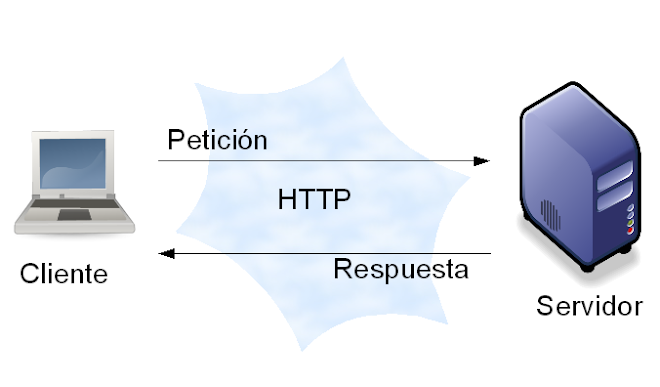
\includegraphics[width=11cm]{figs/client-server.png}
            \caption{Esquema Cliente-Servidor}
            \label{fig:client-server}
\end{figure}

El nombre que tomará dicha aplicación web será \textbf{eOptimizer}, haciendo referencia a su objetivo principal: realizar simulaciones por medio de una optimización. En la Figura~\ref{fig:logo} se muestra el logo creado para la aplicación. Dicho logo ha sido diseñado por el propio alumno y se inspira en el objetivo de eficiencia energética que tiene el sistema.
\begin{figure}[!h]
            \centering
            
\includegraphics[width=4cm]{figs/logo.png}
            \caption{Logo de eOptimizer}
            \label{fig:logo}
\end{figure}

Antes de entrar en la implementación de la aplicación debe definirse correctamente el funcionamiento que ha de tener. Esto implica determinar el flujo posible de interacción de un cliente con la aplicación web, algo que a la hora de implementar la captura de errores o las restricciones facilitará mucho la complejidad de desarrollo. Para ello ha de construirse un \textbf{diagrama de flujo}.\\

Un diagrama de flujo describe un sistema informático, y tiene como objetivo planificar, estudiar y diseñar procesos complejos o algoritmos. De entre todas las funcionalidades que pueden implementar los diagramas de flujo, deben mencionarse:
\begin{itemize}
\item Mostrar la ejecución del código de un software.
\item Facilitar la comprensión de la estructura y funcionalidad de una aplicación web.
\item Explicar visualmente como un usuario puede navegar por una página web.
\item Mostrar el alcance de un sistema.
\end{itemize}
Para crear un diagrama de flujo debe tenerse en cuenta el alcance del sistema. En el caso de este \gls{TFG}, un usuario (rol de cliente) interactuará con la aplicación web (servidor) con el objetivo de realizar una \textbf{simulación} del consumo eléctrico de un día determinado que habría tenido su hogar mediante el sistema propuesto, comparándolo frente a su situación actual, por tanto la entrada al diagrama de flujo debe ser el hecho de acceder a la aplicación web, y la salida será la información obtenida en la simulación realizada.\\

Lo primero que debe hacer un cliente es identificarse, pues en el servidor debe tenerse en cuenta el usuario de la base de datos que está interactuando con el sistema para realizar la simulación, ya que necesita la información asociada. Por ello, el usuario deberá introducir sus credenciales para poder acceder. Si un usuario nunca antes ha accedido a eOptimizer, deberá registrarse.\\

Una vez haya introducido la información de usuario para su registro, esta se insertará en la base de datos y si todo va correctamente, el siguiente paso es introducir la información asociada a su hogar, que será empleada para realizar sus simulaciones. Cuando se haya introducido se insertará en la base de datos, teniendo almacenada toda la información necesaria del usuario en curso, por lo que se permitiría el acceso al índice o \textit{dashboard} de la web.\\

Desde el \textit{dashboard} un usuario podrá realizar simulaciones, introduciendo los datos necesarios para la misma, como son la fecha que desea simular y el fichero de consumo de Endesa de ese día. Si esta información es correcta, el \textit{backend} realizará la optimización obteniendo previamente la información de las APIs AEMET y Esios relativa al día de simulación y mostrando los resultados obtenidos al cliente.\\

En la Figura~\ref{fig:diagrama-flujo} se muestra el diagrama de flujo de la aplicación que permite visualizar todo el funcionamiento de manera mas sencilla. Nótese que en color azul se muestran la entrada y salida del flujo, en color morado se muestran las decisiones, en color amarillo los datos de entrada, en color naranja los procesos y en color verde el acceso a la base de datos.\\
\begin{figure}[H]
            \centering
            \includegraphics[width=15cm]{figs/diagrama_flujo.png}
            \caption{Diagrama de flujo de eOptimizer}
            \label{fig:diagrama-flujo}
\end{figure}

Una vez definido el flujo que debe seguir la aplicación web, el siguiente paso en esta iteración es la implementación del servidor. Para ello se hace uso de \textbf{Flask}~\cite{Grinb14}. Flask es un microframework para desarrollo web con Python. Sigue una filosofía minimalista por la que con un pequeño número de líneas de código se permite crear aplicaciones web. Este framework tiene dos dependencias principales:
\begin{itemize}
\item \textbf{Werkzeug}: Proporciona los componentes necesarios de \textit{routing}, \textit{debugging} y \gls{WSGI}.
\item \textbf{Jinja2}: Proporciona las herramientas para la integración de \textit{templates} html en un servidor Flask.
\end{itemize}
Desafortunadamente Flask no cuenta con soporte nativo para integración con base de datos, pero como se mencionó anteriormente, SQLAlchemy se integra perfectamente con este framework de desarrollo web, por lo que se dispone de todos los componentes necesarios para la creación de la aplicación web. Las buenas prácticas de Flask recomiendan usar \textbf{virtualenv} para la instalación de las dependencias de una aplicación web. Un virtualenv~\cite{VirPy} es una copia privada del intérprete de Python donde se pueden integrar paquetes y librerías sin afectar al entorno del sistema, de manera que permite tener un entorno privado por aplicación web en la misma máquina donde las dependencias de cada aplicación están organizadas en estancos sin afectarse entre sí. Para este \gls{TFG} se ha creado un virtualenv donde mediante el gestor de paquetes de Python3 \textbf{pip3} se han instalado las dependencias necesarias del proyecto. Estas dependencias se han ido mencionando a lo largo de este capítulo (Scipy, SQLAlchemy, Flask, Werkzeug.security, etc) y se encuentran en el fichero \textit{requirements}.\\

En un servidor Flask deben definirse las rutas o \textit{endpoints} que existirán en la aplicación web. La petición de un cliente web a un \textit{endpoint} disparará la ejecución de la función asociada a esa ruta, lo que lo convierte en un framework sencillo pero a la vez muy potente. En la Tabla~\ref{tab:endpoints} se muestran los \textit{endpoints} de la aplicación eOptimizer. Nótese que cada \textit{endpoint} puede recibir un determinado tipo de operación http.
\begin{table}[hp]
        \centering
        \begin{tabular}{|l|c|p{0.5\linewidth}|}
                \hline
                \textbf{\textit{Endpoint}} & \textbf{Operación HTTP} & \textbf{Descripción}\\ \hline
                '/' & GET & Representa el \textit{index} de la aplicación web. Su función será redirigir al formulario de inicio de sesión si no hay usuario identificado o al \textit{dashboard} si hay usuario identificado.\\ \hline
                '/login' & POST & Petición de inicio de sesión con las credenciales de usuario. \\ \hline
                '/logout' & GET & Petición de cierre de sesión del usuario identificado. \\ \hline
                '/signup' & POST & Petición de registro de usuario con la información necesaria. \\ \hline
                '/add-home' & POST & Petición de registro de hogar del usuario identificado proporcionando la información necesaria. \\ \hline
                '/simulation' & POST & Petición de realizar una simulación en el hogar del usuario identificado proporcionando la información necesaria. \\ \hline
                errorhandler(404) & GET & \textit{Hook} de captura de errores cuya labor será redirigir a la página de error cuando se realice una petición a un \textit{endpoint} que no existe. \\ \hline
             \end{tabular}
        \caption{\textit{Endpoints} de la aplicación web}
        \label{tab:endpoints}
\end{table}

Ha de implementarse correctamente el control de sesiones y la autenticación de usuarios. Mediante el módulo del que se habló en el apartado anterior, \textbf{Werkzeug.security}~\cite{Werk} se controla lo relativo a seguridad. Dicho módulo contiene funciones (denominadas \textit{helpers}) para manejo de contraseñas como son \textit{generate\_password\_hash} y \textit{check\_password\_hash}. Nótese como ambas son utilizadas en la clase del modelo \textit{User} (listado~\ref{lst:modelUser}). La primera recibe como argumento una cadena de texto que es la introducida por el nuevo usuario. Esta función genera un \textit{hash} encriptado que almacena en base de datos, de tal forma que la información sensible queda protegida y no es vulnerable. La segunda función es llamada cuando se desea comprobar la veracidad de unas credenciales. Recibe una cadena de texto y comprueba si el \textit{hash} almacenado tras ser desencriptado coincide con dicha cadena de texto. Estas funciones son de gran ayuda a la hora de implementar el inicio de sesión en eOptimizer, pues se comprueba si el email introducido (atributo indizado) existe en base de datos y si es así, se comprueba si la contraseña introducida coincide con la de dicho usuario haciendo uso de esta herramienta. En lo referente al control de sesiones, Flask cuenta con el módulo \textbf{session}, el cuál guarda la información de sesión de un cliente web determinado durante cierto tiempo en el atributo 'logged\_in'. Por lo tanto, la lógica a seguir en el inicio de sesión pasa por comprobar si el usuario con el email introducido existe. Si existe, se comprueba la contraseña introducida mediante el método \textit{check\_password}. Si es correcta, el usuario habría sido autenticado, lo que se traduce en almacenar el objeto \textit{User} en una variable global \textbf{\textit{currentUser}} y dar valor true a \textit{session['logged\_in']}. Por lo tanto, existen tres salidas posibles de login: usuario correcto (éxito), usuario no existe (fallo) y contraseña incorrecta (fallo). Todas las operaciones posteriores que requieran de autenticación comprobarán los valores de esas dos variables.\\

Para realizar una simulación, existen varias estructuras de control que comprueban posibles errores o incompatibilidades antes de efectuarla. Si todo es correcto, se instancia un objeto de la clase Simulation proporcionándole los objetos \textit{Home} y \textit{User} relativos al usuario autenticado además de la fecha que se desea simular y el fichero de consumo obtenido de Endesa. El valor de retorno de llamar a la función \textit{optimize} de ese objeto Simulation es un json que contiene los valores obtenidos en parejas clave-valor.\\

Los valores de retorno de los métodos asociados a cada \textit{endpoint} llaman a la función auxiliar de Flask \textbf{render\_template}. Esta función emplea las utilidades de Jinja2 y muestra al cliente la plantilla html definida en la función.
Los posibles errores son acumulados en una lista \textit{errors}, la cuál es enviada como argumento a \textbf{render\_template}. Esto es debido a una funcionalidad que integra Jinja2, que permite insertar código en una plantilla html, pudiendo mostrar variables, implementar estructuras de control, bucles, etc. De esta forma el \gls{JSON} obtenido de la simulación se consigue mostrar correctamente en el \textit{frontend}. El Listado~\ref{lst:loginErrors} contiene el proceso de mostrar los posibles errores producidos en el formulario de inicio de sesión haciendo uso de esta funcionalidad.
\begin{lstlisting}[language=Html,float=ht,caption={Muestreo de errores en el formulario de inicio de sesión},label={lst:loginErrors}]

<div class="alert alert-danger" role="alert">
  {{ error }}
</div>

\end{lstlisting}

Al levantar un servidor Flask, este recibe la configuración pertinente de un fichero. En este \gls{TFG} se proporciona mediante \textit{prod\_config} o \textit{test\_config}. Cada uno de ellos levanta una instancia diferente de la aplicación. El primero enlaza el servidor de Flask con la base de datos de producción, y el segundo con la base de datos de test. Para poner en funcionamiento una instancia del servidor se ha implementado la clase \textit{run}, mostrada en el Listado~\ref{lst:runModule}. En él se maneja la app mediante el módulo \textit{Manager} de \textit{flask\_script} que permite manejar un servidor de desarrollo de una aplicación Flask. La configuración de producción mencionada anteriormente es aplicada a app, para despues instanciar la base de datos y ejecutar el \textit{create\_all} del que se habló anteriormente. A partir de ahí el servidor estará ejecutándose y listo para recibir peticiones.

\begin{lstlisting}[language=Python,float=ht,numbers=none,caption={Módulo \textit{run} para arrancar el servidor},label={lst:runModule}]
#!/usr/bin/python3
# -*- coding: utf-8; mode: python -*-

from flask_script import Manager
from flask_sqlalchemy import SQLAlchemy
from app import app, db
from config import prod_config
from models import Base

# Deploy to production
manager = Manager(app)
app.config.from_object(prod_config)
db = SQLAlchemy(app)
Base.metadata.create_all(bind=db.engine)

if __name__ == '__main__':
    manager.run()
\end{lstlisting}

\subsection{\textit{Frontend} de la aplicación web}
Para la implementación del \textit{frontend} y desarrollo web se ha utilizado la librería \textbf{Bootstrap}~\cite{Boots}. Esta librería proporciona un conjunto de herramientas para crear sitios web \textit{responsives} y livianos. Entre estas herramientas se encuentran clases html predefinidas, funciones de Javascript, etc. Esto ha permitido una base sobre la que trabajar para construir el sitio web. Se han implementado las siguientes plantillas html:
\begin{itemize}
\item \textbf{Base}: Contiene el encabezado y el pie de página de la web y es heredada en el resto de plantillas.
\item \textbf{Login}: Vista que muestra el formulario de inicio de sesión y el de nuevo usuario en eOptimizer. Da como resultado la ejecución del \textit{endpoint} asociado '/login' o '/signup', devuelto condicionalmente mediante las herramientas de Jinja2 explicadas anteriormente.
\item \textbf{New\_home}: Vista que muestra el formulario de introducción de datos asociados al hogar del usuario. Como resultado se ejecuta el método del \textit{endpoint} asociado '/add-home', que inserta en base de datos la información proporcionada.
\item \textbf{Dashboard}: Vista principal de eOptimizer una vez autenticado. Cuenta con una tabla de información acerca de la información del hogar correspondiente y con un formulario para realizar simulaciones (Figura~\ref{fig:dashboard}).
\item \textbf{Simulation}: Vista de reporte de una simulación. Una vez es realizada la optimización, la función \textit{render\_template} carga esta vista procesando la información del json obtenido (Figura~\ref{fig:simulationView}, donde se muestra esta vista de la simulación del 16 de Abril de 2019). Contiene tres funcionalidades: mostrar la tabla de distribución de la energía, mostrar la tabla de precios que se dieron el día simulado, y por último descargar el fichero de reporte de simulación.
\item \textbf{Not\_found}: Vista que se muestra cuando el \textit{hook} errorhandler captura una ruta no existente. Informa del error y da opción de volver al \textit{dashboard}.
\end{itemize}
\begin{figure}[H]
            \centering
            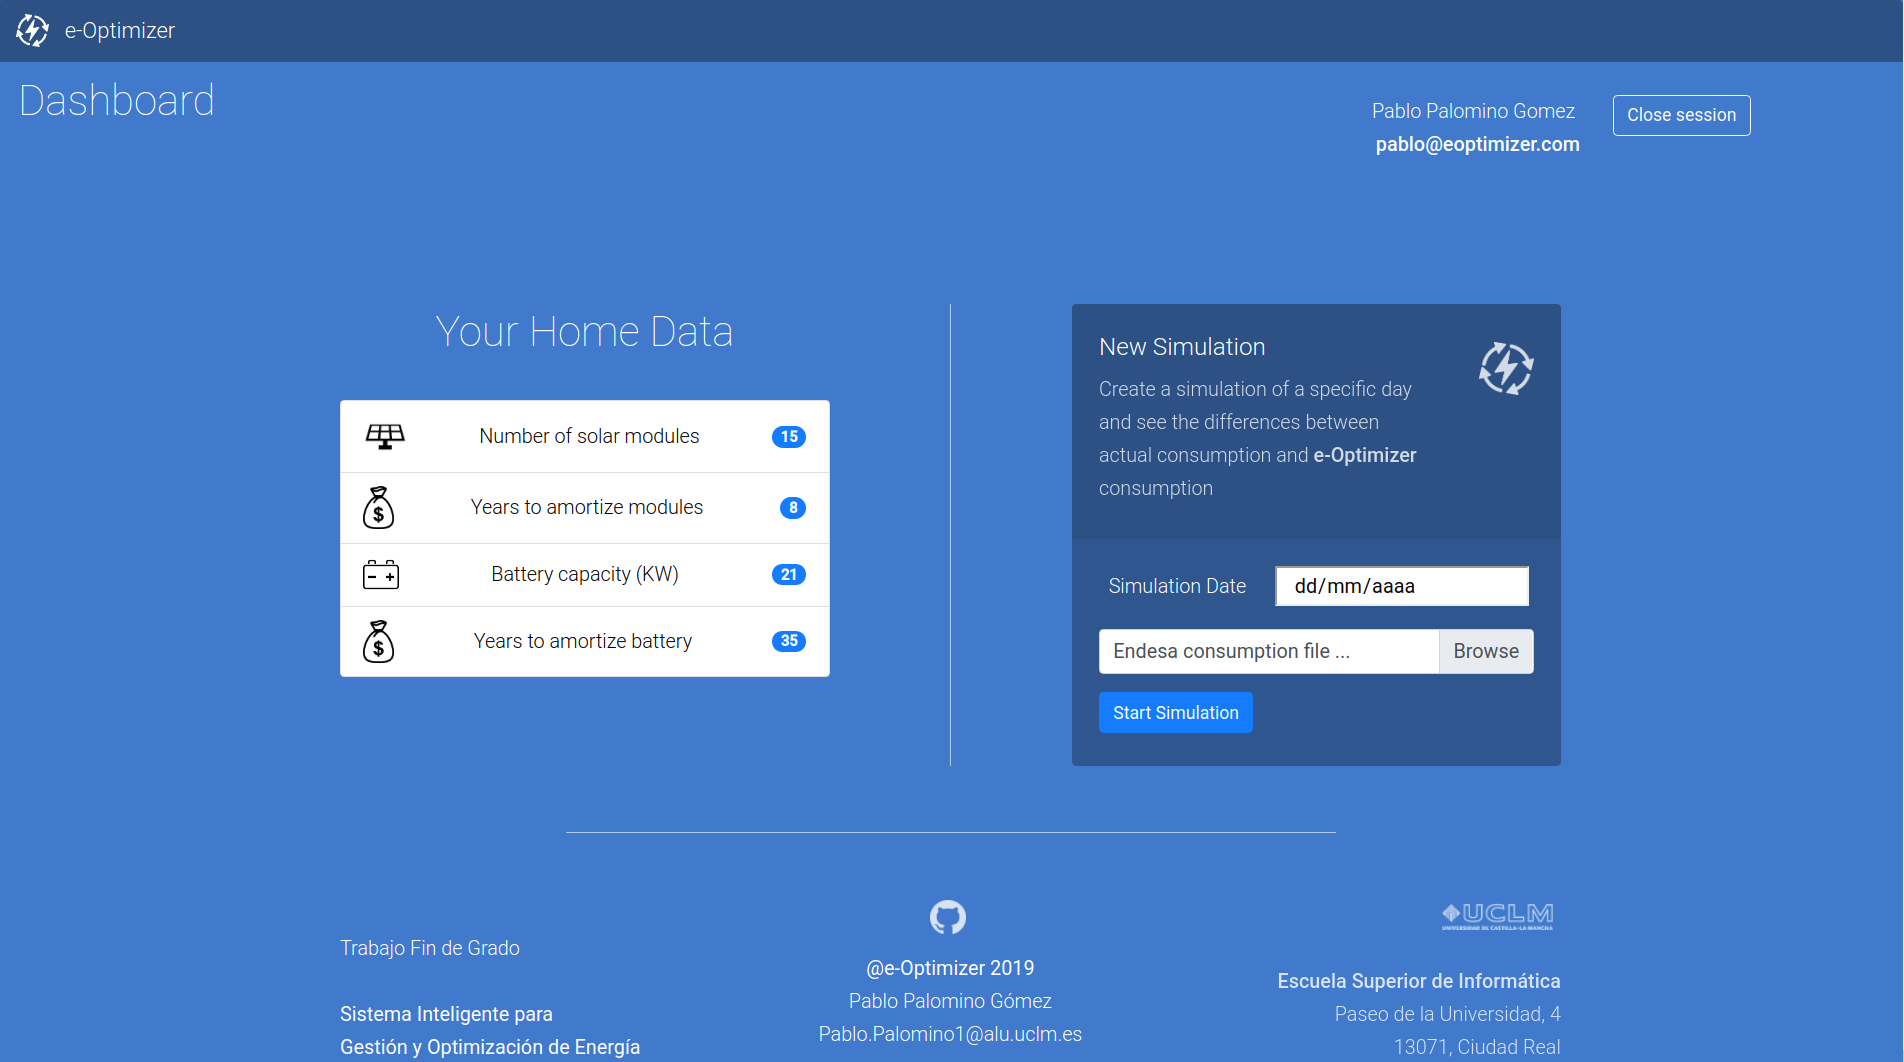
\includegraphics[width=17cm]{figs/dashboard.png}
            \caption{Vista \textit{dashboard} de la aplicación}
            \label{fig:dashboard}
\end{figure}
\begin{figure}[H]
            \centering
            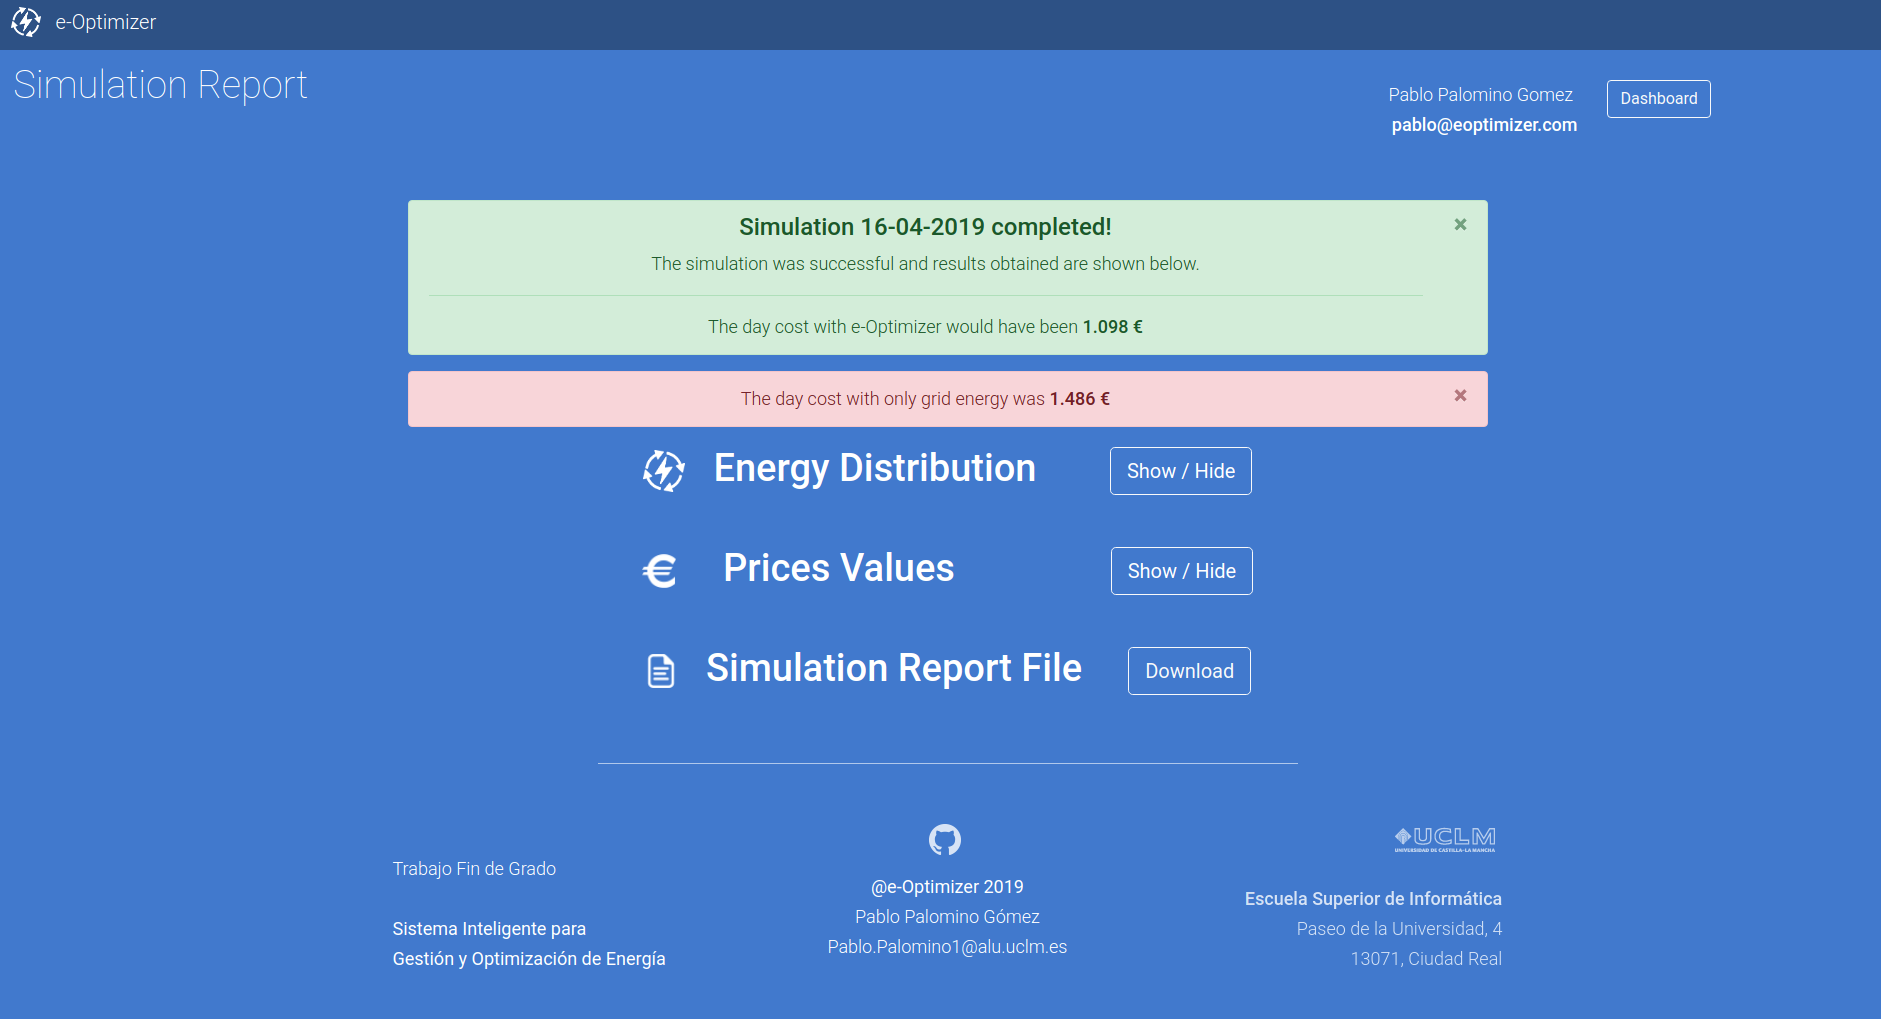
\includegraphics[width=17cm]{figs/simulation.png}
            \caption{Vista \textit{simulation report} de la aplicación}
            \label{fig:simulationView}
\end{figure}

En el listado~\ref{lst:simulationReport} del Anexo A se mostró el resultado de una simulación durante la Iteración 4 (Sección~\ref{sec:hito4}). Dicha información corresponde con el fichero de reporte de simulación, que a partir de ahora se puede descargar en la vista Simulation (Figura~\ref{fig:simulationView}). Además la información de la simulación es procesada por horas en la tabla \textbf{energy distribution}, que mediante funciones de javascript muestra barras de distribución de la energía por horas, con el fin de facilitar la comprensión del usuario y hacerlo más visible. Véase la Figura~\ref{fig:energyDistrib}, donde se muestra la tabla en las horas comprendidas entre la 13:00 y las 23:00 de la optimización del día 16 de Abril de 2019.
\begin{figure}[H]
            \centering
            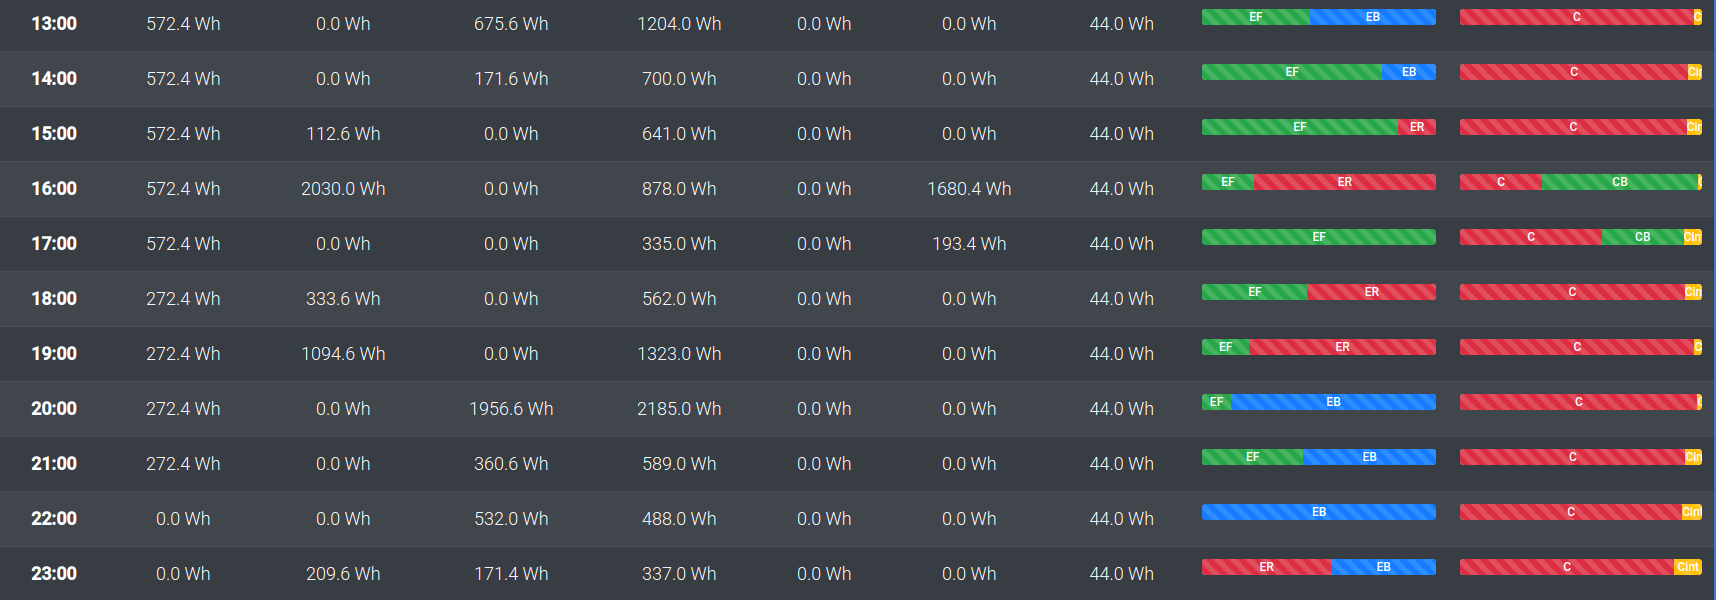
\includegraphics[width=17cm]{figs/energy_distrib.png}
            \caption{Tabla \textit{energy distribution} del 16/04 entre 13:00-23:00}
            \label{fig:energyDistrib}
\end{figure}


Como salida de esta iteración se obtiene la versión totalmente funcional de la aplicación web integrada con el \textit{backend} para optimizar simulaciones. Actualmente solo es posible ejecutarlo en la máquina local, siendo dependiente del software y dependencias propios de la misma. En la siguiente iteración se buscará la integración en la nube de la aplicación. Los tests relativos a la aplicación web (\textit{routing} y vistas) que demuestran la correcta funcionalidad se detallan en el Anexo B.
